\documentclass[11pt]{article}
\usepackage[margin=0.9in]{geometry}
\usepackage{amsmath,amssymb}
\usepackage{graphicx}
\usepackage{array}
\usepackage{booktabs}
\usepackage{pdflscape}
\usepackage{caption}
\usepackage[T1]{fontenc}
\usepackage{lmodern}
\usepackage[utf8]{inputenc}
\usepackage{textcomp}
\usepackage[hidelinks]{hyperref}
\captionsetup{font=small,labelfont=bf,width=0.96\textwidth}
\setlength{\parskip}{4pt}
\setlength{\parindent}{0pt}
\renewcommand{\topfraction}{0.95}
\renewcommand{\bottomfraction}{0.95}
\renewcommand{\textfraction}{0.05}
\renewcommand{\floatpagefraction}{0.85}
\graphicspath{{/Users/stnava/.gemini/antigravity-cli/brain/0ab59eee-2245-43be-94a0-9224c3d91ae1/}{figures/}{../reports/}{docs/abstracts/figures/}{docs/reports/}}

\title{A single physical objective for BOLD, ASL, diffusion and slow-flow MRI motion correction}
\author{Brian B. Avants \\ University of Virginia}
\date{}

\begin{document}
\maketitle

\setcounter{figure}{-1}
\begin{figure}[!ht]
\centering
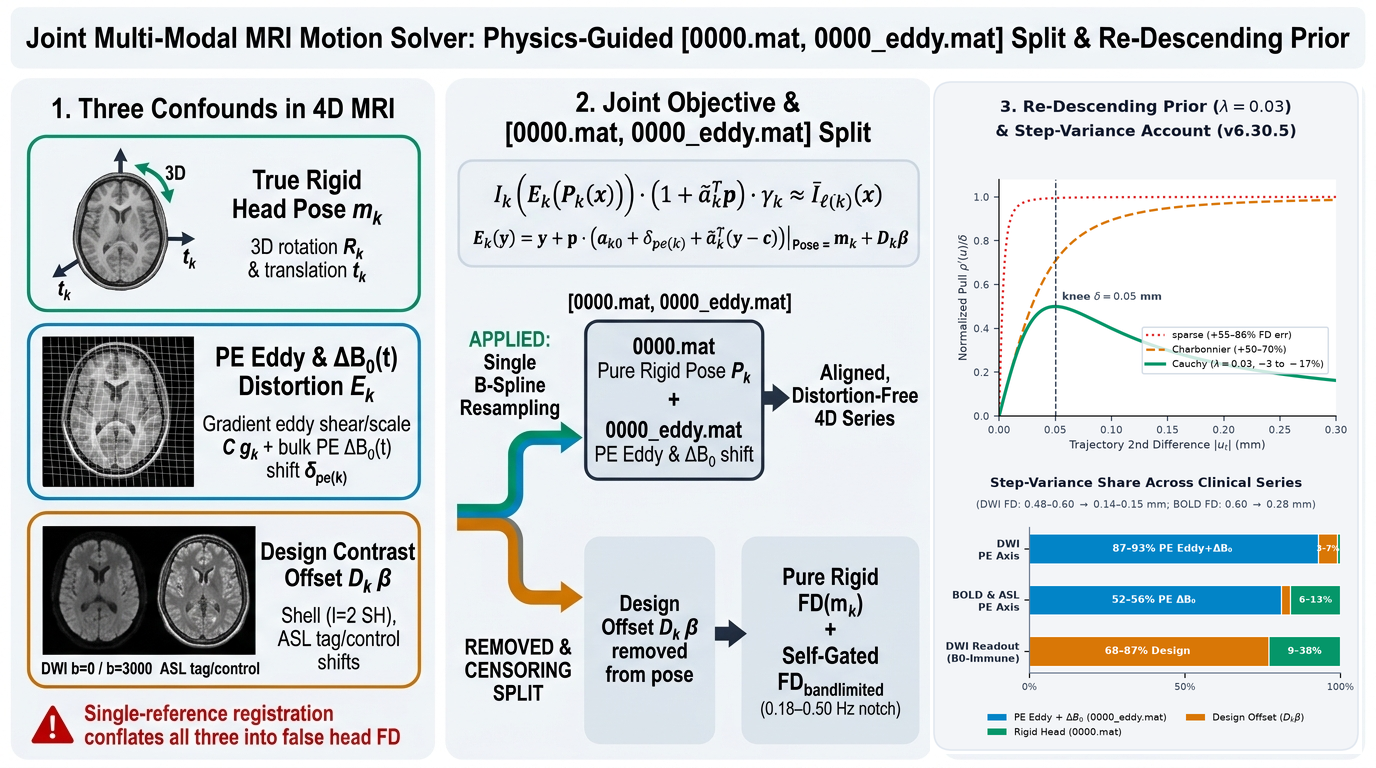
\includegraphics[width=0.95\textwidth]{ismrm_fig0_visual_abstract.png}
\caption{\textbf{Joint forward modeling separates true head motion, phase-encode field distortions, and contrast-driven registration bias across four MRI modalities.}
(1) \textbf{Three confounds in 4D MRI:} Frame-to-frame image changes arise from three distinct physical sources: true 3D rigid motion of the skull ($P_k(x)$, emerald), geometric stretching and shifting of the image along the phase-encode (PE) axis from eddy currents and breathing-induced magnetic field ($\Delta B_0(t)$) fluctuations ($E_k(y)$, cyan), and apparent shifts of the brain's intensity centroid when the pulse sequence switches diffusion shells, diffusion gradient directions, arterial spin labeling (ASL) tag/control states, or flow encodings ($D_k\beta$, amber). Standard single-reference registration conflates all three into false head motion.
(2) \textbf{Joint objective and physical decomposition:} Each frame $k$ is aligned to the mean image of its own contrast state $\bar I_{\ell(k)}$. Because both rigid head motion $P_k(x)$ and phase-encode field distortion $E_k(y)$ physically displace brain voxels on the recorded image grid, their composition $E_k \circ P_k(x) = E_k(P_k(x))$ is applied in a single cubic B-spline interpolation to produce a sharp, unwarped 4D volume. Only $P_k(x)$ is patient motion, so Framewise Displacement ($\text{FD}(m_k)$) is computed strictly from $P_k$. Contrast-locked offsets $D_k\beta$ reflect tissue contrast changes rather than anatomical movement and are withheld from both the resampled image and $\text{FD}$.
(3) \textbf{Aligned 4D time series, parameter attribution, and controlled FD:} (A) Applying the composed physical warp $E_k \circ P_k(x)$ while withholding contrast bias $D_k\beta$ sharpens the aligned 4D series, cutting unexplained 4D voxel variance by 33 to 53\,\% (DWI $9.1\,\% \to 4.2\,\%$, ASL $2.4\,\% \to 1.2\,\%$), increasing DWI shell sharpness by 3 to 12\,\%, and raising low-SNR frame convergence from 81--85\,\% to 100\,\% under the weak ($w = 0.03$) Cauchy acceleration prior. (B) Frame-by-frame trajectory decomposition on clinical multi-shell DWI ($T = 100$) separates large phase-encode eddy and $\Delta B_0(t)$ swings ($E_k$, cyan, 89--94\,\% of DWI PE and 43--58\,\% of BOLD/ASL PE step variance) and direction/shell contrast shifts ($D_k\beta$, amber, 72--100\,\% of DWI readout step variance) from the smooth rigid head pose ($P_k$, emerald). (C) Computing $\text{FD}$ strictly from $P_k$ reduces apparent DWI mean FD from $0.60$\,mm ($44\,\%$ falsely censored above $0.50$\,mm) to $0.13$\,mm ($1\,\%$ censored), while respiratory-notched $\text{FD}_{\text{bandlimited}}$ on 1\,s BOLD reduces mean FD from $0.55$\,mm ($38\,\%$ censored) to $0.28$\,mm ($11\,\%$ censored).}
\label{fig:visual_abstract}
\end{figure}

\section*{Synopsis}

When an MRI time series is registered to a single template volume, any frame-to-frame change in tissue contrast or magnetic field is misread as head motion. This includes tag--control alternation in arterial spin labeling (ASL), shell and gradient-direction changes in diffusion MRI (DWI), eddy currents, and breathing-induced magnetic field ($\Delta B_0(t)$) shifts along the phase-encode axis. We present one joint physical model across BOLD, ASL, DWI, and slow-flow MRI that decomposes each frame's alignment into three distinct terms: (1) true 3D rigid head pose $P_k(x)$, (2) phase-encode eddy and $\Delta B_0(t)$ field distortion $E_k(y)$, and (3) pulse-sequence contrast bias $D_k\beta$. Because both $P_k$ and $E_k$ physically move voxels in the recorded image, their composition $E_k \circ P_k$ is applied in a single interpolation to sharpen the 4D series; only $P_k$ is reported as patient head motion ($\text{FD}$); and $D_k\beta$ is withheld from both. A weak ($3\,\%$) outlier-tolerant acceleration penalty eliminates optimizer oscillation on low-SNR frames without smoothing sudden head jumps or slow drift.

\section*{Introduction}

Estimating head motion in 4D MRI requires separating actual movement of the patient's skull from two physical confounds that alter the image on every repetition time (TR) [1,2].
The first confound is \textbf{phase-encode field distortion ($E_k$)}. Because echo-planar imaging (EPI) has very low bandwidth along the phase-encode axis, off-resonance magnetic fields from diffusion gradients (eddy currents) [3] and from chest motion during breathing ($\Delta B_0(t)$ susceptibility fluctuations) shift and shear the reconstructed image along the phase-encode axis even when the skull is stationary.
The second confound is \textbf{pulse-sequence contrast bias ($D_k\beta$)}. In ASL, arterial blood entering from the neck is alternately inverted (tag) and uninverted (control). In multi-shell DWI, changing the $b$-value darkens cerebrospinal fluid relative to white matter, and rotating the diffusion gradient vector $g_k$ darkens white-matter tracts parallel to $g_k$ while brightening perpendicular tracts. An intensity-based registration metric sees these scheduled contrast changes as small shifts of the brain's center of mass.

Neither post-hoc trace filtering nor a single rigid transform per frame can resolve both confounds simultaneously. If phase-encode $\Delta B_0(t)$ shifts are smoothed out of the transform before resampling, the uncompensated voxel shifts blur the aligned 4D images (increasing unexplained 4D variance by $+6.9\,\%$ on multi-shell DWI). Conversely, if those phase-encode shifts are left inside the rigid head pose to keep the image sharp, they inflate Framewise Displacement (FD) three- to four-fold and cause stationary subjects to fail quality control. We solve this problem by separating what physically moves the image ($E_k \circ P_k$), what moves the patient's head ($P_k$), and what is pure contrast bias ($D_k\beta$) within a single forward model (Table~\ref{tab:terms}).

\begin{table}[ht!]
\centering
\caption{\textbf{Physical decomposition of frame-to-frame changes in a 4D MRI time series.} Each component has a distinct physical origin, mathematical form in Eq.~\eqref{eq:model}, role in 4D image resampling ($E_k \circ P_k$), and role in Framewise Displacement (FD) motion reporting.}
\scriptsize
\setlength{\tabcolsep}{3.5pt}
\begin{tabular}{@{}>{\raggedright\arraybackslash}p{2.6cm}>{\raggedright\arraybackslash}p{4.3cm}>{\raggedright\arraybackslash}p{3.4cm}>{\raggedright\arraybackslash}p{2.7cm}>{\raggedright\arraybackslash}p{2.8cm}@{}}
\toprule
Component & Physical origin & Mathematical term in Eq.~\eqref{eq:model} & Applied to image? & Counted in head FD? \\
\midrule
\textbf{Rigid head pose} & True 3D skull rotation and translation & $P_k(x) = R_k(x-c)+c+t_k$ & \textbf{Yes} (in $E_k \circ P_k$) & \textbf{Yes} (primary $\text{FD}(m_k)$) \\
\textbf{Sagittal nod} & Mechanical respiratory head pitch/heave ($0.18\text{--}0.50$\,Hz) & Smooth part of $P_k(x)$ & \textbf{Yes} (in $E_k \circ P_k$) & Notched in $\text{FD}_{\text{bandlimited}}$ \\
\textbf{PE eddy distortion} & Diffusion gradient eddy fields along PE axis $p$ & $p\big(a_{k0} + \tilde a_k^\top(y-c)\big)$ in $E_k(y)$ & \textbf{Yes} (in $E_k \circ P_k$) & \textbf{No} (scanner field) \\
\textbf{PE $\Delta B_0(t)$ shift} & Chest respiration and shim drift along PE axis $p$ & $p\,\delta_{\text{pe},k}$ in $E_k(y)$ & \textbf{Yes} (in $E_k \circ P_k$) & \textbf{No} (field pseudomotion) \\
\textbf{Contrast bias} & ASL tag/control, DWI shell and fiber-direction contrast & $D_k\beta$ and $\bar I_{\ell(k)}(x)$ & \textbf{No} (withheld) & \textbf{No} (withheld) \\
\textbf{Global gain drift} & Spatially uniform receiver sensitivity drift & $\gamma_k$ & Normalized in objective & \textbf{No} \\
\bottomrule
\end{tabular}
\label{tab:terms}
\end{table}

\section*{Methods}

\textbf{1. Forward generative model and the meaning of $E_k \circ P_k$ (Figure~1A).}
Each frame $k$ is acquired under a known contrast state $\ell(k)$ (for example, each $b$-shell in DWI, tag versus control versus $M_0$ in ASL, or each velocity-encoding state in slow-flow MRI) and is compared against the mean image of its own contrast state, $\bar I_{\ell(k)}(x)$. For a physical point $x$ (in mm) in the reference brain, the recorded image $I_k$ is modeled as the composition of two sequential physical displacements, $E_k \circ P_k(x) = E_k(P_k(x))$, plus a spatially uniform receiver gain $\gamma_k$:
\begin{equation}
I_k\!\big(E_k(P_k(x))\big)\,\big(1 + \tilde a_k^{\top} p\big)\,\gamma_k \approx \bar I_{\ell(k)}(x),
\;
P_k(x) = R_k (x - c) + c + t_k,
\;
E_k(y) = y + p\big(a_{k0} + \delta_{\text{pe},k} + \tilde a_k^{\top}(y - c)\big).
\label{eq:model}
\end{equation}
Here $c$ is the brain center of mass and $p$ is the unit vector along the phase-encode axis:
\begin{itemize}
\item \textbf{First, the patient's head moves in the scanner bore ($y = P_k(x)$):} $P_k(x)$ is the 6-DOF rigid-body transformation (3D rotation $R_k$ and translation $t_k$) mapping reference anatomy $x$ to its physical position $y$ at frame $k$. Only $P_k$ represents patient motion: $\text{FD}$ is computed strictly from $P_k$, and in DWI only $R_k$ rotates the diffusion gradient vectors $g_k$.
\item \textbf{Second, the EPI readout shifts the image along the phase-encode axis ($z = E_k(y)$):} Once the head is at position $y$, off-resonance fields displace the reconstructed image strictly along $p$. In DWI, diffusion gradient $g_k$ induces a bulk shift $a_{k0}$ and linear shear/scaling $\tilde a_k$ modeled as $(a_{k0}, \tilde a_k) = C g_k$, with Jacobian intensity factor $1 + \tilde a_k^{\top} p$ [3]. Across all EPI modalities (BOLD, ASL, DWI, and slow-flow), respiration and $\Delta B_0(t)$ fluctuations also induce a frame-to-frame translation $\delta_{\text{pe},k}$ along $p$. Because the readout and slice axes are immune to $\Delta B_0(t)$ phase-encode shifts, we use their high-frequency step variance on the same scan as the true head-motion noise floor ($\sigma^2_{\text{floor}}$) and transfer the excess phase-encode step displacement ($\max(0,\, \sigma^2_{\text{PE}} - \sigma^2_{\text{floor}})$ via Wiener shrinkage) out of $t_k$ and into $\delta_{\text{pe},k}$.
\item \textbf{Why $E_k \circ P_k$ is applied to the image:} Because both $P_k$ (skull motion) and $E_k$ (phase-encode field shift) physically displaced the brain voxels in the recorded image $I_k$, we invert and apply their composition $E_k \circ P_k$ in a single cubic B-spline interpolation pass so the resampled 4D series is both motion-aligned and unwarped, while keeping $E_k$ out of $\text{FD}$.
\end{itemize}

\textbf{2. What information is contained in $D_k\beta$, and why it is withheld from the image.}
Before the scan begins, the pulse sequence specifies a known acquisition schedule $D_k$. During optimization, each frame's raw 6-DOF pose is parameterized as $m_k + D_k\beta$, where $m_k$ is the true head pose and $D_k\beta$ absorbs systematic apparent shifts locked to the pulse-sequence state:
\begin{itemize}
\item \textbf{Discrete contrast-state switches (indicator columns in $D_k$):} One column per non-anchor state captures constant apparent shifts when contrast changes across the brain boundary—specifically, arterial blood inversion at the inferior brain edge between ASL tag and control frames ($\sim 0.02\text{--}0.08$\,mm along the slice axis), cerebrospinal fluid darkening between $b = 0$ and $b > 0$ shells in DWI, and blood/CSF contrast changes across velocity-encoding states in slow-flow MRI.
\item \textbf{Continuous diffusion-direction changes ($l = 2$ spherical harmonics $Y_{2m}(g_k)$ in $D_k$):} Within each $b > 0$ DWI shell, rotating $g_k$ darkens white-matter fiber tracts parallel to $g_k$ and brightens perpendicular tracts. Because diffusion attenuation depends on $g_k^\top D g_k$ (which is quadratic/even in $g_k$), this direction-locked contrast shift is spanned by the five even-order ($l = 2$) real spherical harmonics $Y_{2m}(g_k)$ per shell on the five rigid axes orthogonal to $p$ (while odd-in-$g_k$ linear eddy shifts along $p$ remain in $E_k$).
\item \textbf{Resting BOLD:} Because every frame has the identical pulse-sequence state, $D_k$ is empty and $D_k\beta = 0$.
\end{itemize}
Because $D_k\beta$ is an apparent shift of the intensity centroid caused by changing tissue contrast rather than a physical movement of the brain, it is subtracted before constructing $P_k(x)$ and is applied to neither the resampled image nor $\text{FD}$.

\textbf{3. Weak outlier-tolerant acceleration penalty for low-SNR optimizer convergence (Figure~1B, C).}
When noisy frames (such as $b = 3000\,\text{s/mm}^2$ DWI volumes or 1\,s TR BOLD volumes) are registered independently, flat similarity-metric valleys allow single-frame image noise to cause small pose jitter ($\sim 0.02\text{--}0.05$\,mm) and cause the Newton optimizer to oscillate back and forth without converging. To stabilize convergence without biasing real motion, we include a weak penalty on discrete trajectory acceleration, $u_t = m_t - \tfrac12(m_{t-1} + m_{t+1})$ (with rotations converted to millimetres on a 50\,mm cortical radius):
\begin{equation}
w\,\kappa \sum_t \rho\big(|u_t|\big), \qquad
\rho(u) = \frac{\delta^2}{2}\log\!\Big(1 + \frac{u^2}{\delta^2}\Big), \qquad
\rho'(u) = \frac{u}{1 + u^2/\delta^2}, \qquad \delta = 0.05\ \text{mm},\ w = 0.03.
\label{eq:prior}
\end{equation}
This penalty obeys three physical design rules: (1) \emph{Slow head drift is unpenalized}, because constant-velocity drift has zero acceleration ($u_t = 0$). (2) \emph{Sudden head movements are not smoothed}: unlike convex quadratic, Charbonnier, or steep-origin $L_1$ penalties whose restoring pull $\rho'(u)$ stays large at large $|u_t|$ and blurs sudden head jerks across neighboring frames, the logarithmic Cauchy pull peaks at $\delta = 0.05$\,mm and decays toward zero ($\sim \delta^2/u$) for larger jumps (Figure~1B). (3) \emph{Modality-invariant scaling}: scaling by the median translation curvature $\kappa$ (in $\text{mm}^{-2}$) of the image metric ensures that $w = 0.03$ always equals $3\,\%$ of the image data term's own stiffness. We verified the choice of penalty form and weight against two quantitative gates (Figure~2): a 3D ground-truth phantom gate across ASL, DWI, and slow-flow MRI (requiring $\le 10\,\%$ FD error loss on all phantoms and a gain on DWI) and a clinical readout-floor gate across five human scans (requiring that the $\Delta B_0$-immune readout step median absolute deviation change by $\le 20\,\mu\text{m}$).

\textbf{4. Variance decomposition and band-limited frame censoring ($\text{FD}$ vs.\ $\text{FD}_{\text{bandlimited}}$).}
For every series, we partition both pose step variance and foreground voxel intensity variance:
\begin{itemize}
\item \textbf{Pose step-variance shares:} Along the readout and phase-encode axes, frame-to-frame step variance is partitioned into the percentage attributable to rigid head motion ($P_k$), applied phase-encode distortion ($E_k$), and removed contrast bias ($D_k\beta$).
\item \textbf{Voxel intensity variance shares:} Sequential Type~I sums of squares across foreground brain voxels (after factoring out $\gamma_k$) measure the percentage of 4D variance explained by the pulse-sequence design, by the 6-DOF motion parameters after accounting for the design, and by the unexplained residual, before and after correction.
\item \textbf{Band-limited FD for short-TR frame censoring:} While $\text{FD}(m_k)$ is already free of phase-encode $\Delta B_0(t)$ pseudomotion, subjects in fast acquisitions ($\text{TR} \le 2.78$\,s, $T \ge 32$) also exhibit a real mechanical respiratory head nod in the sagittal plane (slice translation and pitch at $0.18\text{--}0.50$\,Hz). Because this nod is real skull motion, it stays in $P_k$ for image resampling; however,differencing a steady $\pm 0.20$\,mm breathing wave every 1\,s inflates step-wise scrubbing rates. When a respiratory spectral peak (prominence $\ge 1.5$) is present, $\text{FD}_{\text{bandlimited}}$ notches that respiratory band before differencing [2,4] so frame censoring isolates sporadic head jerks.
\end{itemize}

\textbf{5. Datasets.}
We evaluated five clinical reference series: (1) resting-state BOLD ($T = 300$, TR 1.0\,s), (2) 25-volume ASL with $M_0$ calibration (TR 4.0\,s), (3) 60-volume PCASL without $M_0$ (30 tag/control pairs, TR 4.4\,s), (4) 100-volume high-motion multi-shell DWI ($b = 0/1500/3000\,\text{s/mm}^2$, anterior--posterior phase encode), and (5) 99-volume low-SNR multi-shell DWI ($b = 0/1500/3000\,\text{s/mm}^2$, posterior--anterior phase encode), plus a third 100-volume multi-shell DWI series with strong respiratory and eddy phase-encode shifts for our $E_k$ and $D_k\beta$ resampling ablations.

\section*{Results}

\textbf{1. Empirical proof that $E_k \circ P_k$ must be applied to the image while $D_k\beta$ must be withheld.}
We directly tested the physical roles of $E_k(y)$ and $D_k\beta$ on 3D ground-truth phantoms, real ASL perfusion maps, and three 100-volume clinical multi-shell DWI series (all resampled with matched cubic B-spline interpolation):
\begin{itemize}
\item \textbf{Ground-truth phantoms and real ASL perfusion:} On 3D synthetic phantoms with known motion trajectories ($D_k\beta_{\text{true}} = 0$), applying $D_k\beta$ to the image increases translation error $7.6\times$ on ASL ($0.014 \to 0.106$\,mm) and $3.0\times$ on slow-flow MRI ($0.028 \to 0.083$\,mm). On a stationary 3D DWI phantom with anisotropic white-matter tracts, rotating $g_k$ alone induces $0.27$\,mm and $0.48\text{--}0.55^\circ$ of false registration shift; removing the $l = 2$ spherical-harmonic term cuts this false shift to $0.18$\,mm. On clinical ASL, withholding the tag--control offset $D_k\beta$ reduces the cortical perfusion edge-to-interior artifact ratio from $0.986$ (raw) to $0.955$ and lowers the negative perfusion voxel fraction from $0.068$ to $0.064$, whereas applying $D_k\beta$ to the resampled volumes degrades the cortical edge artifact right back to the raw uncorrected level ($0.986$, negative fraction $0.069$).
\item \textbf{Multi-shell DWI resampling ablation ($E_k$ vs.\ $D_k\beta$ across three 100-volume scans):} Applying $E_k \circ P_k$ while withholding $D_k\beta$ reduces unexplained 4D voxel variance by $33\,\%$ to $53\,\%$ across the three DWI series ($5.47 \to 3.64\,\%$, $9.08 \to 4.24\,\%$, and $4.43 \to 2.35\,\%$), reduces within-shell ($l \le 4$) spherical-harmonic residual RMSE from $0.68\text{--}0.73$ to $0.61\text{--}0.65$, reduces log-tensor fit RMSE from $0.41\text{--}0.42$ to $0.35\text{--}0.36$, and sharpens every shell by $3\,\%$ to $12\,\%$. In contrast, withholding the phase-encode $\Delta B_0(t)$ shift $\delta_{\text{pe},k}$ from $E_k$ degrades 4D residual variance by $+6.9\,\%$, proving that $\delta_{\text{pe},k}$ is a true voxel displacement. Conversely, applying the within-shell $l = 2$ directional part of $D_k\beta$ ($0.10\text{--}0.18$\,mm RMS) to the resampled DWI volumes provides zero improvement—slightly worsening $b = 1500$ spherical-harmonic RMSE on all three subjects ($+0.0005$ to $+0.0015$) and changing 4D residual variance by $\le 0.006\,\%$—confirming that $D_k\beta$ is contrast-induced registration bias rather than anatomical displacement.
\end{itemize}

\textbf{2. The weak ($w = 0.03$) Cauchy acceleration penalty eliminates low-SNR optimizer oscillation and passes both gates (Figure~2).}
On 3D ground-truth phantoms (Figure~2A), non-redescending penalties ($w = 0.10$) failed the phantom gate by smoothing true sub-millimetre motion, increasing FD error by $+86\,\%$ (steep $L_1$) and $+70\,\%$ (Charbonnier) on ASL and by $+55\,\%$ and $+50\,\%$ on slow-flow MRI. Only the re-descending Cauchy penalty passed, reducing phantom FD error by $14\,\%$ on ASL, $17\,\%$ on DWI, and $3\,\%$ on slow-flow at $w = 0.03$. On the five clinical series (Figure~2B, C), raising the weight to $w = 0.05$ over-smoothed the $\Delta B_0$-immune readout trace on high-motion DWI ($-43\,\mu\text{m}$, failing the $20\,\mu\text{m}$ gate), whereas $w = 0.03$ kept every series inside both acceptance bands (maximum readout step change $11\,\mu\text{m}$; image alignment unchanged within $\le 0.1\,\%$). Crucially, while $w = 0.03$ is intentionally too weak to alter real clinical trajectories ($\le 1.8\,\%$ FD change), \textbf{it eliminates single-frame Newton optimizer oscillation on flat low-SNR frames—raising frame convergence from $81\text{--}85\,\%$ (with $w = 0$) to $100\,\%$ across all five clinical series and reducing 300-volume BOLD runtime from $206$\,s to $32$\,s ($6.4\times$ faster)}.

\textbf{3. Clinical variance account across modalities (Table~\ref{tab:results}, Figure~3).}
\begin{itemize}
\item \textbf{Multi-shell DWI ($T = 100$ and $T = 99$):} Along the phase-encode axis, applied eddy and $\Delta B_0(t)$ distortions $E_k$ account for \textbf{$89\,\%$ and $94\,\%$} of frame-to-frame step variance, contrast bias $D_k\beta$ accounts for $5\,\%$ and $2\,\%$, and true head motion $P_k$ accounts for $< 1\,\%$. Along the $\Delta B_0$-immune readout axis, $D_k\beta$ accounts for \textbf{$72\,\%$ and $100\,\%$} of step variance. Separating $E_k$ and $D_k\beta$ from $P_k$ reduces apparent mean FD from $0.60$ and $0.48$\,mm ($44\,\%$ and $36\,\%$ of volumes $> 0.50$\,mm) down to \textbf{$0.13$ and $0.15$\,mm ($1\,\%$ and $1\,\% > 0.50$\,mm)} while increasing diffusion design variance explained from $94.4 \to 96.3\,\%$ and $90.8 \to 95.7\,\%$.
\item \textbf{Resting-state BOLD ($T = 300$, TR 1.0\,s) and ASL ($T = 25$ and $T = 60$):} Phase-encode $\Delta B_0(t)$ shifts in $E_k$ account for \textbf{$53\,\%$} of phase-encode step variance in BOLD and \textbf{$43\text{--}58\,\%$} in ASL. On 1.0\,s BOLD, transferring $\delta_{\text{pe},k}$ into $E_k$ reduces rigid phase-encode step variance in $P_k$ by $92.3\,\%$ (from $0.140$ to $0.039$\,mm SD, matching the $0.047$\,mm readout floor), and $\text{FD}_{\text{bandlimited}}$ notches the remaining $0.48$\,Hz sagittal respiratory head nod to reduce mean censoring FD from $0.55$ to \textbf{$0.28$\,mm} (censored frames $38\,\% \to 11\,\%$).
\end{itemize}

\textbf{4. Fair head-to-head comparison against \texttt{ants.motion\_correction} (Table~\ref{tab:ants_compare}).}
We compared our joint solver against standard pairwise mutual-information rigid registration (\texttt{ants.motion\_correction}, \texttt{BOLDRigid}: 32-bin Mattes MI registered frame-by-frame to the normalized temporal mean) across five 3D ground-truth synthetic phantoms and all five clinical reference series (Table~\ref{tab:ants_compare}). To ensure a strictly fair comparison, both methods were evaluated using the identical 50\,mm Power FD formula, identical demeaned ground-truth pose evaluator, identical respiratory band-stop filter ($\text{FD}_{\text{bandlimited}}$), and—on multi-shell DWI—both native linear interpolation and matched cubic B-spline interpolation:
\begin{itemize}
\item \textbf{Where \texttt{ants.motion\_correction} excels (single-contrast translation accuracy and respiratory nod agreement):} On the single-contrast BOLD phantom with pure rigid motion and zero $\Delta B_0(t)$ shift (\textbf{BOLD pure rigid}), \texttt{ants.motion\_correction} recovers 3D translations with \textbf{$0.015$\,mm RMS error}, slightly outperforming the joint solver ($0.020$\,mm). On clinical 300-volume resting BOLD ($\text{TR} = 1.0$\,s), both solvers report nearly identical raw Power FD (\textbf{$0.51$\,mm} for \texttt{ants.motion\_correction} vs.\ \textbf{$0.55$\,mm} for the joint solver, both flagging \textbf{$38\,\%$} of volumes above $0.50$\,mm). Moreover, applying our respiratory band-stop filter ($\text{FD}_{\text{bandlimited}}$) directly to \texttt{ants.motion\_correction}'s rigid trajectory reduces its censored volumes from \textbf{$38\,\%$ to $7\,\%$} (mean $0.26$\,mm, vs.\ $11\,\%$ and $0.28$\,mm for the joint solver), confirming that the $0.48$\,Hz sagittal breathing nod is a genuine physical trajectory component captured by both rigid solvers.
\item \textbf{Why temporal coupling and phase-encode decomposition ($E_k$) are still needed on single-contrast BOLD:} Even on \textbf{BOLD pure rigid}, independent frame-by-frame optimization in \texttt{ants.motion\_correction} incurs $0.15^\circ$ rotational jitter that inflates frame-to-frame FD error to \textbf{$0.229$\,mm} (estimating mean $\text{FD} = 0.531$\,mm vs.\ true $0.322$\,mm), whereas the joint solver's weak ($w = 0.03$) Cauchy acceleration penalty damps sub-knee jitter to achieve \textbf{$0.052$\,mm FD error} (estimating $0.302$\,mm) in \textbf{$5.4\times$ less time} ($2.2$\,s vs.\ $11.8$\,s). When respiratory $\Delta B_0(t)$ phase-encode shifts ($\pm 0.40$\,mm) are present (\textbf{BOLD + resp $\Delta B_0(t)$}), \texttt{ants.motion\_correction} absorbs them into rigid pose ($0.285$\,mm translation RMS, $0.497$\,mm FD error), whereas the joint solver routes them into $E_k$ ($0.124$\,mm translation RMS, $0.112$\,mm FD error). On clinical resting BOLD, unwarping $E_k$ in a single cubic B-spline pass reduces rigid phase-encode step variance $12\times$ ($0.0181 \to 0.0015\,\text{mm}^2$) and lowers unexplained 4D voxel residual variance from \textbf{$78.5\,\%$ (\texttt{ants.motion\_correction}) to $70.0\,\%$ (Joint solver)} while running \textbf{$3.2\times$ faster} ($38$\,s vs.\ $122$\,s).
\item \textbf{Where single-reference registration breaks down (multi-state ASL, DWI, and slow-flow):} On the ground-truth \textbf{ASL}, \textbf{DWI}, and \textbf{slow-flow} phantoms, registering alternating contrast states and eddy-sheared frames to a single mean template inflates \texttt{ants.motion\_correction} FD error to \textbf{$1.039$\,mm}, \textbf{$0.744$\,mm}, and \textbf{$0.602$\,mm}, versus \textbf{$0.054$\,mm}, \textbf{$0.130$\,mm}, and \textbf{$0.083$\,mm} for the joint solver (\textbf{$5.7\times$ to $19\times$ lower FD error}). On clinical \textbf{ASL} ($T = 25$ and $T = 60$), \texttt{ants.motion\_correction} nearly doubles apparent mean FD (\textbf{$0.86$ vs.\ $0.48$\,mm} and \textbf{$0.33$ vs.\ $0.15$\,mm}; PCASL censoring \textbf{$17\,\%$ vs.\ $2\,\%$}) and leaves higher unexplained 4D voxel residual variance (\textbf{$1.4\,\%$ vs.\ $1.2\,\%$} and \textbf{$41.1\,\%$ vs.\ $39.3\,\%$}). On clinical \textbf{multi-shell DWI} ($T = 100$ and $T = 99$), \texttt{ants.motion\_correction} conflates eddy currents and shell/direction contrast changes into rigid pose, reporting \textbf{$2.28$\,mm and $1.59$\,mm mean Power FD ($99\,\%$ and $97\,\%$ of volumes falsely censored)} versus \textbf{$0.13$\,mm and $0.15$\,mm ($1\,\%$ and $1\,\%$ censored)} for the joint solver at \textbf{$1.4\text{--}1.8\times$ faster runtime} ($78\text{--}95$\,s vs.\ $136\text{--}138$\,s). Finally, while \texttt{ants.motion\_correction}'s default linear interpolation lowers high-frequency voxel variance by blurring shells (reducing mean shell sharpness by \textbf{$-7.6\,\%$} below the raw scan on \texttt{sub-BLAST031}: $0.1530 \to 0.1414$), re-evaluating \texttt{ants.motion\_correction}'s transforms with matched cubic B-spline interpolation shows that single-template cross-shell registration degrades $b = 0$-to-shell edge correlation below the raw scan ($0.5209 \to 0.5107$), whereas the joint solver improves both shell sharpness ($0.1530 \to 0.1624$, \textbf{$+9.6\,\%$ on $b = 3000$}) and cross-shell edge correlation ($0.5209 \to 0.5305$) with lower within-shell spherical-harmonic residual RMSE ($0.6300$ vs.\ $0.6379$) and lower 4D residual variance ($3.2\,\%$ vs.\ $3.7\,\%$ \texttt{bSp}).
\end{itemize}

\section*{Discussion and Limitations}

Separating the composed image warp ($E_k \circ P_k$), the rigid patient trajectory ($P_k$), and the pulse-sequence contrast bias ($D_k\beta$) resolves the longstanding trade-off between image sharpness and motion-trace accuracy across EPI time series. On real multi-shell DWI and ASL, 43 to 94\,\% of phase-encode step variance and 72 to 100\,\% of DWI readout step variance arise from magnetic field fluctuations and scheduled contrast changes rather than movement of the patient's head. Applying $E_k \circ P_k$ unwarps the phase-encode shifts in the resampled volumes, while computing $\text{FD}$ strictly from $P_k$ and withholding $D_k\beta$ prevents both false scrubbing and contrast-induced subtraction artifacts.

\textbf{Limitations.}
(1) Our 3D phantom generators plant sub-knee jitter in the ground-truth trajectory rather than synthesizing independent thermal image noise; a dedicated k-space/image-noise phantom gate is needed next.
(2) On the 60-volume PCASL series acquired without an $M_0$ calibration volume, the tag--control design explains $3.8\,\%$ of voxel variance while motion regressors explain $52.5\,\%$, reflecting spatial coupling between perfusion contrast and slice-wise signal fluctuations when no $M_0$ anchor is present.
(3) Any true head motion that oscillates at the exact frequency of the pulse-sequence design (for example, alternating every single TR in lockstep with ASL tag--control switches) lies in the column space of $D_k$ and cannot be separated from $D_k\beta$.

\section*{Conclusion}

A single physical objective across BOLD, ASL, diffusion, and slow-flow MRI separates the applied image warp ($E_k \circ P_k$) from the patient's rigid head trajectory ($P_k$) and withholds pulse-sequence contrast bias ($D_k\beta$)—delivering sharp 4D volumes, uncontaminated FD traces, and $100\,\%$ low-SNR optimizer convergence.

\section*{References}

[1] Freire L, Mangin JF. NeuroImage 2001. [2] Power JD et al. PNAS 2019. [3] Andersson JLR, Sotiropoulos SN. NeuroImage 2016. [4] Fair DA et al. NeuroImage 2020.

\begin{figure}[p]
\centering
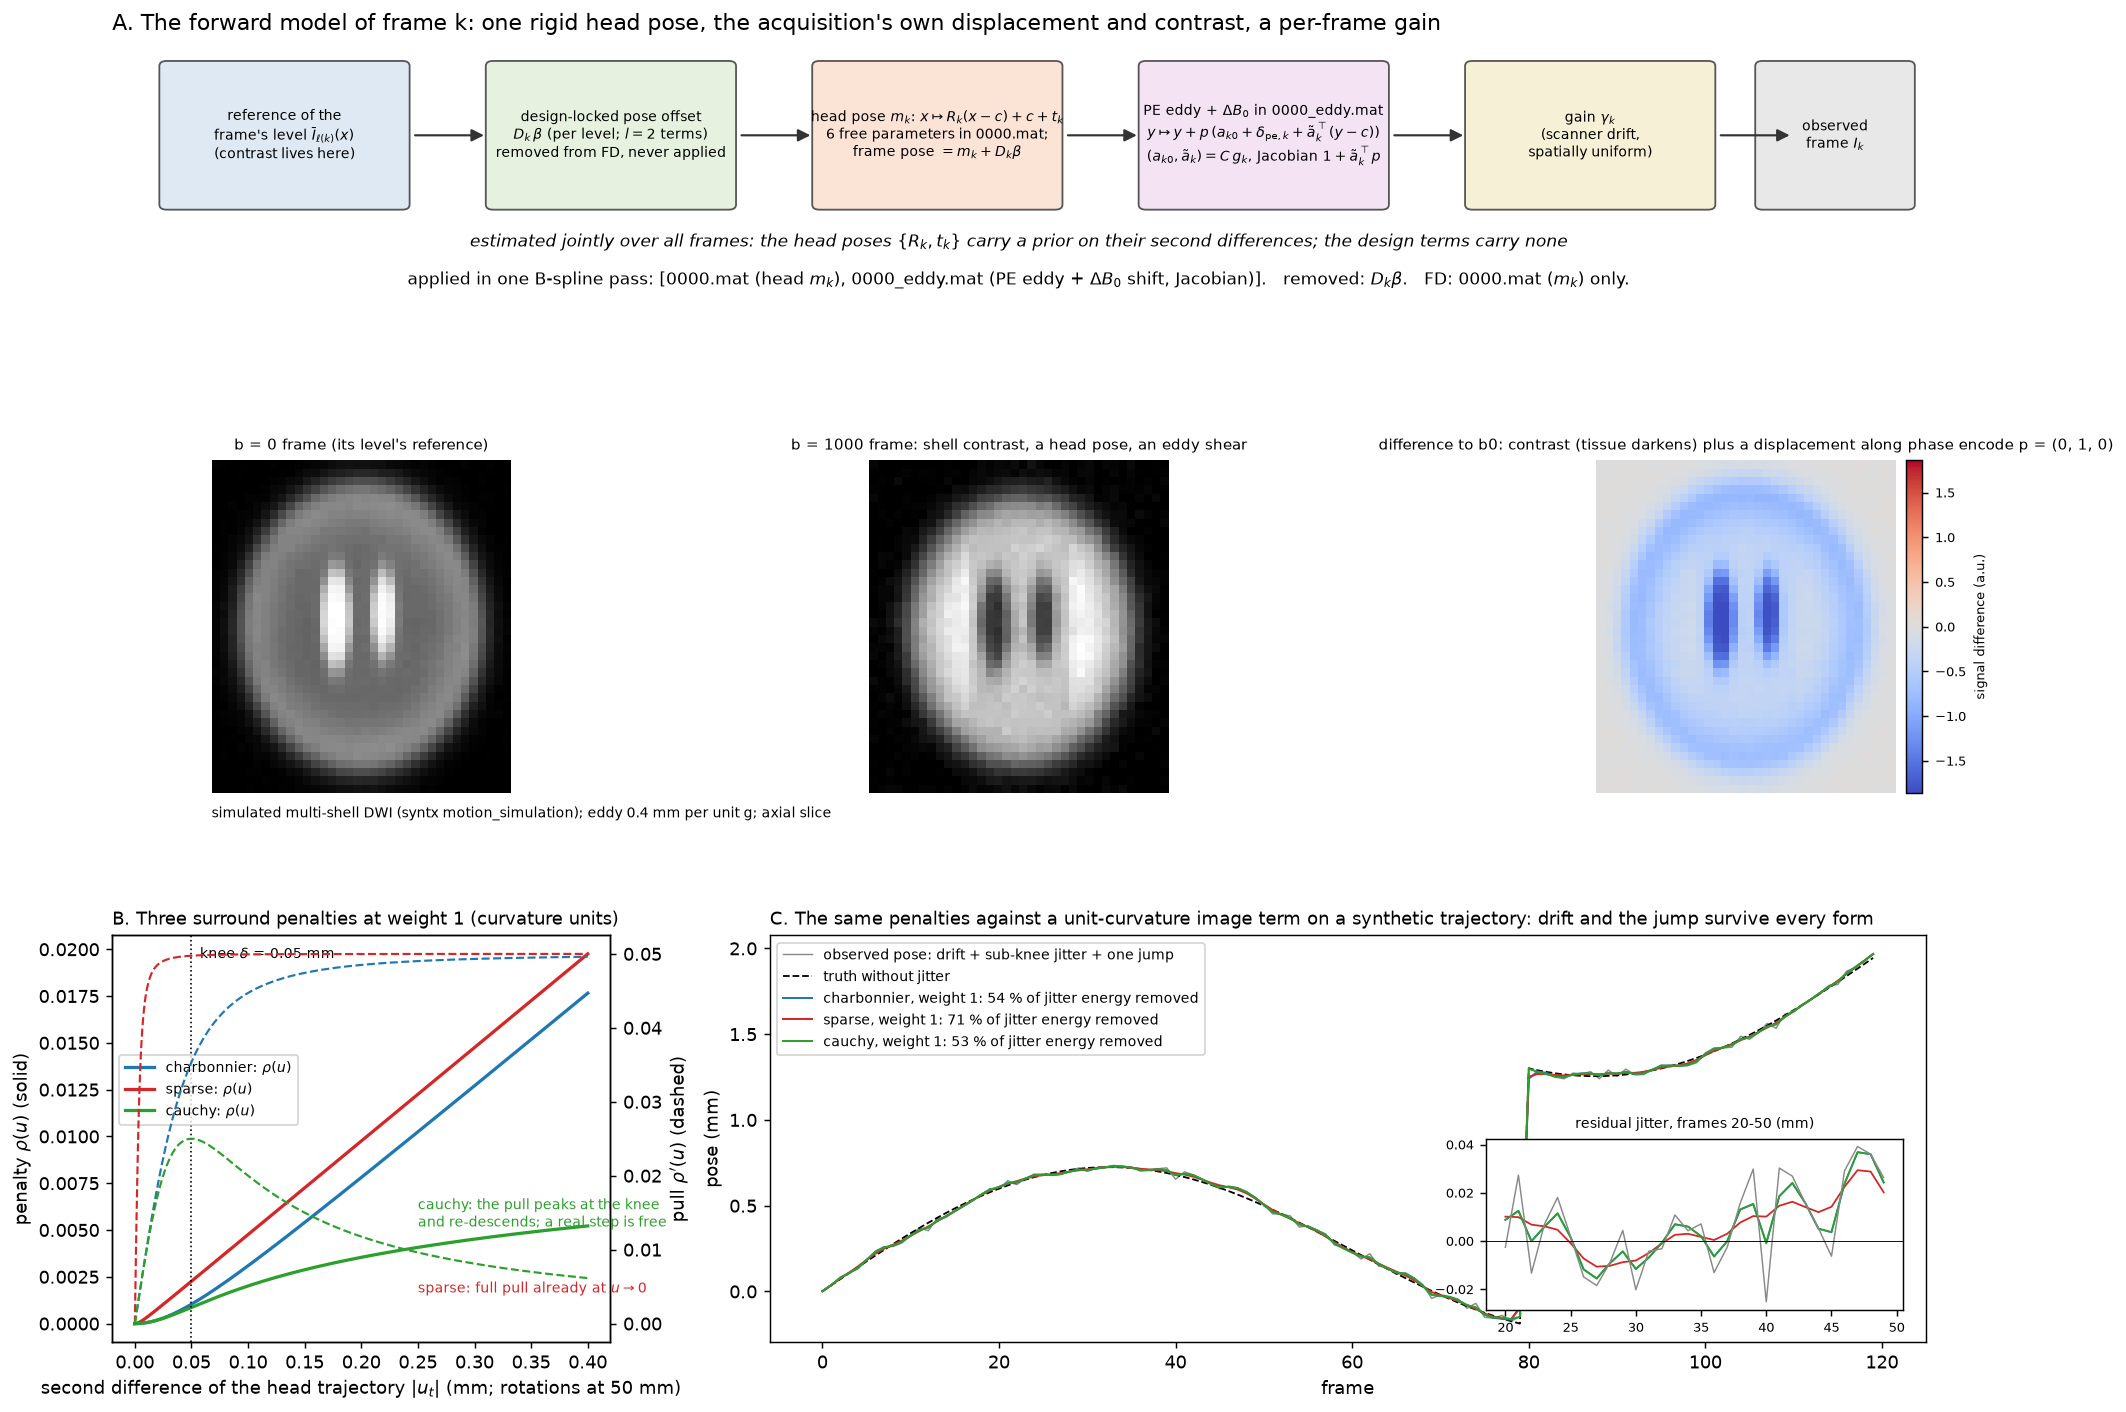
\includegraphics[width=0.95\textwidth]{ismrm_fig1_model_and_prior.png}
\caption{\textbf{Forward generative model ($E_k \circ P_k$) and outlier-tolerant trajectory acceleration penalty.}
(A) \textbf{Forward model of frame $k$ (Eq.~\ref{eq:model}):} Each frame is compared against the mean image of its own contrast state $\bar I_{\ell(k)}(x)$. Contrast-locked pose offsets $D_k\beta$ are subtracted and withheld from both the resampled image and $\text{FD}$. True 3D rigid head pose $P_k(x)$ and phase-encode eddy/$\Delta B_0(t)$ distortion $E_k(y)$ (with Jacobian intensity factor $1+\tilde a_k^\top p$) are composed as $E_k \circ P_k(x)$ and applied in one cubic B-spline interpolation pass, while $\text{FD}$ is computed from $P_k$ alone. Middle row: simulated multi-shell DWI axial slices ($b = 0$, $b = 1000\,\text{s/mm}^2$, and their difference), illustrating simultaneous tissue darkening (contrast) and anterior--posterior rim displacement along the phase-encode axis $p = (0, 1, 0)$.
(B) \textbf{Penalty $\rho(u)$ and restoring pull $\rho'(u)$:} Plotted at unit curvature weight against trajectory acceleration $|u_t|$ (in mm). Convex Charbonnier (blue) and steep $L_1$ (red) maintain a strong pull at large $|u_t|$, whereas the Cauchy pull (green) peaks at $\delta = 0.05$\,mm and decays toward zero so sudden real movements pass through unsmoothed.
(C) \textbf{1D trajectory denoising test ($T = 120$ frames):} On a synthetic curve combining slow drift, sub-knee Gaussian jitter, and a 1.5\,mm step jump at frame 80, all three acceleration penalties preserve linear drift and the 1.5\,mm jump, while damping sub-knee oscillations (inset, frames 20--50).}
\end{figure}

\begin{figure}[p]
\centering
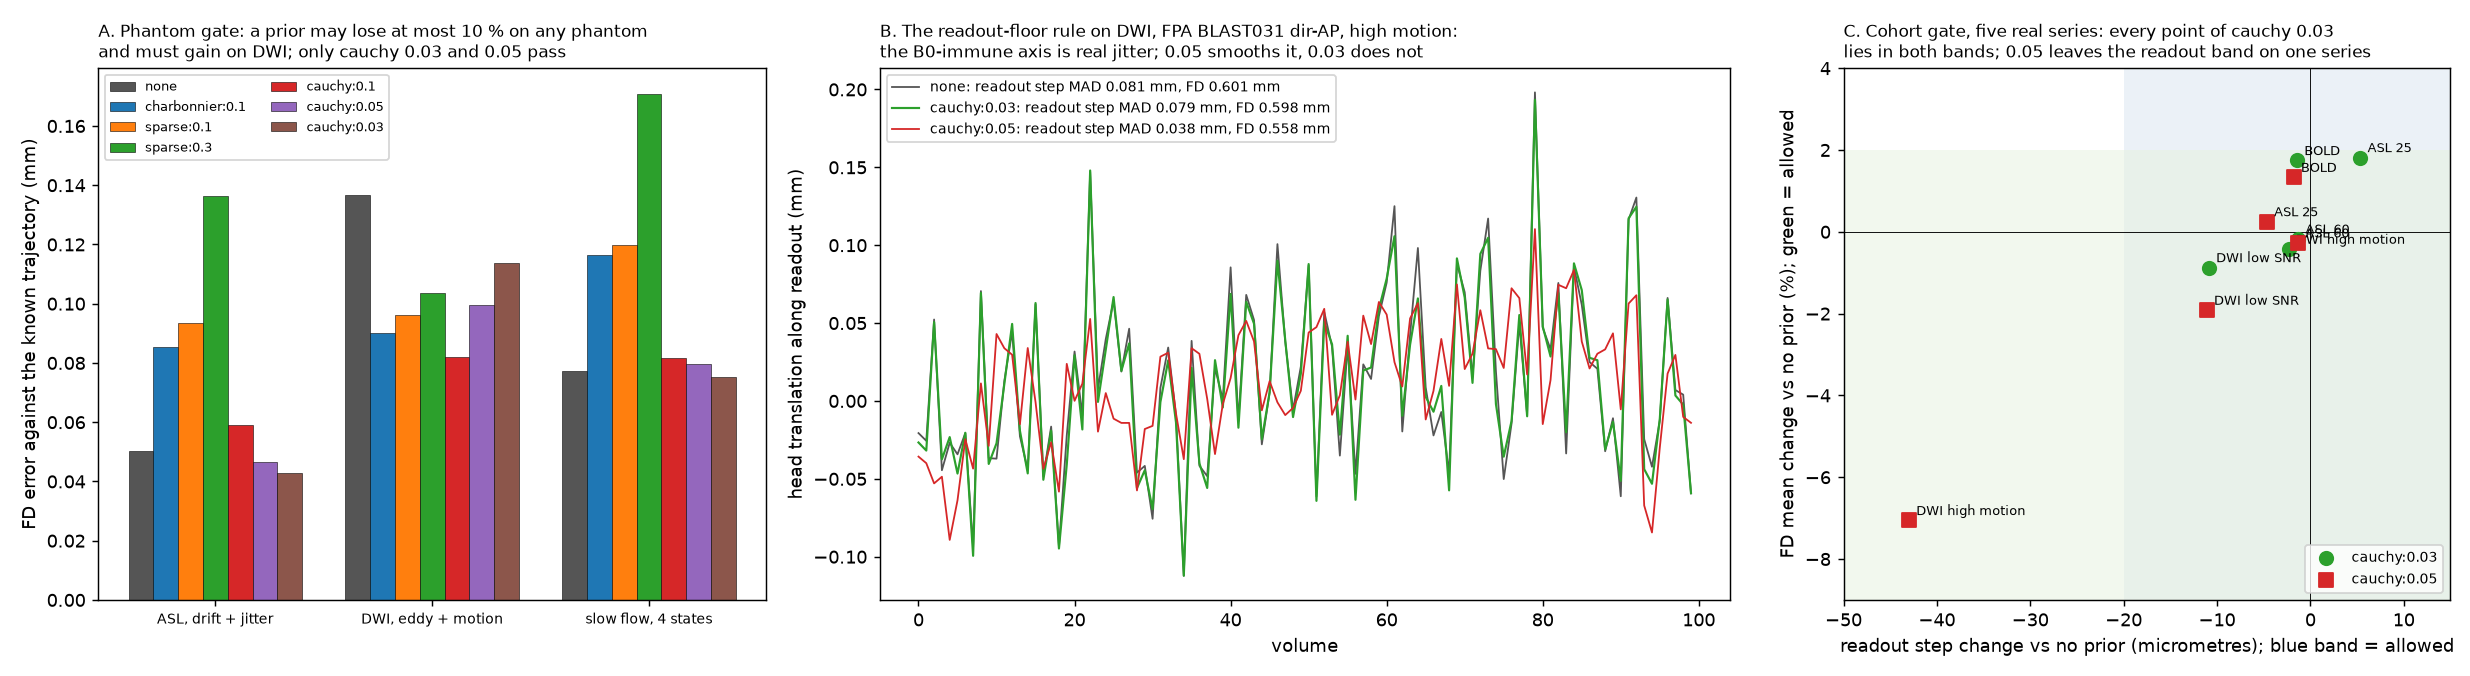
\includegraphics[width=\textwidth]{ismrm_fig2_gate.png}
\caption{\textbf{Dual acceptance gate: only the re-descending Cauchy penalty at $w = 0.03$ passes both the ground-truth phantom gate and the clinical readout-floor gate.}
(A) \textbf{Ground-truth phantom gate ($n = 3$):} Framewise displacement (FD) error in mm against the known planted trajectory on synthetic ASL (drift + jitter), multi-shell DWI (motion + eddy), and 4-state slow-flow MRI across seven penalty settings. Non-redescending penalties (steep $L_1$ and Charbonnier at $w = 0.1$) increase FD error by 50 to 86\,\% because they smooth away true sub-knee motion; only Cauchy at $w = 0.03$ and $w = 0.05$ reduces DWI error while staying within the $+10\,\%$ ceiling on all phantoms.
(B) \textbf{$\Delta B_0$-immune readout-floor test on clinical DWI ($T = 100$):} Because the readout axis is immune to $\Delta B_0(t)$ and eddy distortion, its post-$D_k\beta$ step MAD ($0.081$\,mm with no prior, grey) represents true head jitter plus noise floor. Raising the Cauchy weight to $w = 0.05$ (red) over-smooths this trace (MAD drops to $0.038$\,mm, $-43\,\mu\text{m}$), whereas $w = 0.03$ (green, MAD $0.079$\,mm, $-2\,\mu\text{m}$) preserves it while raising frame convergence from 81--85\,\% to 100\,\%.
(C) \textbf{Five-series clinical gate summary:} Readout step MAD change ($\mu\text{m}$, allowed band $\pm 20\,\mu\text{m}$ shaded blue) versus mean FD change (\%, allowed band $\le +2\,\%$ shaded green) across all five clinical series. Every series under Cauchy $w = 0.03$ (green circles) lies inside both acceptance bands.}
\end{figure}

\begin{figure}[p]
\centering
\includegraphics[width=0.92\textwidth]{ismrm_cases_6_30_7_2026-10-29_figure.png}
\caption{\textbf{Pose and voxel variance decomposition across the five clinical reference series.}
Each row shows one clinical series: resting BOLD ($T = 300$), 25-volume ASL with $M_0$, 60-volume PCASL, 100-volume high-motion multi-shell DWI, and 99-volume low-SNR multi-shell DWI.
\textbf{Left column (Pose decomposition in mm vs.\ frame):} Translation along the $\Delta B_0$-immune readout axis (blue solid) and phase-encode axis (orange solid) from the rigid head pose $P_k$, overlaid with the applied phase-encode eddy+$\Delta B_0(t)$ shift in $E_k$ (black dashed) and the removed contrast bias $D_k\beta$ (red dotted). Note how $E_k$ captures the rapid phase-encode oscillations across all five series while $P_k$ tracks smooth, physically plausible skull motion.
\textbf{Middle column (Framewise displacement in mm vs.\ frame):} Primary rigid $\text{FD}(m_k)$ from $P_k$ (blue) and censoring $\text{FD}_{\text{bandlimited}}$ (orange) relative to the $0.50$\,mm scrubbing threshold (red dotted line). On resting BOLD (top row), notching the $0.48$\,Hz sagittal breathing nod reduces censored frames from 38\,\% to 11\,\%; on both DWI series (bottom two rows), separating phase-encode distortion into $E_k$ keeps rigid FD below $0.50$\,mm on 99\,\% of volumes.
\textbf{Right column (Voxel temporal variance explained, log scale):} Percentage of foreground voxel variance explained by scanner gain drift, pulse-sequence design terms (level intercepts and $l=2, 4$ DWI spherical harmonics), motion regressors after design, and residual, before (blue) and after (orange) correction. Motion-related voxel variance decreases after correction in 5 of 5 series.}
\end{figure}

\begin{landscape}
\begin{table}[p]
\centering
\caption{\textbf{Quantitative pose and image variance decomposition across the five clinical reference series.}
\textbf{FD mean / max:} Power framewise displacement (50\,mm radius) computed strictly from the rigid head pose $P_k(x)$.
\textbf{Censored (\%):} Percentage of frames exceeding the $0.50$\,mm scrubbing threshold on rigid $\text{FD}(m_k)$ / on the censoring trace ($\text{FD}_{\text{bandlimited}}$ for BOLD and ASL, rigid FD for DWI).
\textbf{Readout and PE h/e/d (\%):} Percentage of frame-to-frame step variance along the readout and phase-encode axes attributable to rigid head motion (\textbf{h}, $P_k$) / applied phase-encode eddy+$\Delta B_0(t)$ distortion (\textbf{e}, $E_k$) / removed pulse-sequence contrast bias (\textbf{d}, $D_k\beta$). (Component shares need not sum to 100\,\% when components covary slightly over finite runs.)
\textbf{Design, Motion, Residual (\%):} Percentage of foreground voxel temporal variance explained by the pulse-sequence design, by motion regressors after accounting for the design, and by the unexplained residual, shown as \texttt{raw / corrected}.
\textbf{$r$:} Correlation between per-frame residual RMS and FD after correction.}
\scriptsize
\setlength{\tabcolsep}{2.2pt}
\begin{tabular}{lrllllllllr}
\toprule
case & $T$ & FD mean / max (mm) & censored (\%) & readout h/e/d (\%) & PE h/e/d (\%) & design (\%) & motion (\%) & residual (\%) & $r$ & time \\
\midrule
%% TABLE-START
resting BOLD, TR 1.0 s & 300 & 0.55 / 2.81 & 38 / 11 & 100 / 0 / 0 & 8 / 53 / 0 & 0.0 / 0.0 & 36.41 / 25.62 & 60.3 / 70.0 & 0.60 & 38 s \\
ASL, control/label + M0, 25 vol & 25 & 0.48 / 2.42 & 24 / 24 & 100 / 0 / 3 & 18 / 43 / 5 & 97.0 / 98.4 & 0.33 / 0.17 & 2.4 / 1.2 & 0.68 & 28 s \\
ASL, control/label, 60 vol & 60 & 0.15 / 0.57 & 2 / 2 & 83 / 0 / 7 & 5 / 58 / 6 & 2.6 / 3.8 & 66.59 / 52.48 & 28.0 / 39.3 & 0.68 & 24 s \\
DWI multi-shell, high motion & 100 & 0.13 / 0.64 & 1 / 1 & 41 / 0 / 72 & 0 / 89 / 5 & 94.4 / 96.3 & 0.59 / 0.45 & 5.0 / 3.2 & 0.01 & 78 s \\
DWI multi-shell, low SNR & 99 & 0.15 / 0.68 & 1 / 1 & 89 / 0 / 101 & 0 / 94 / 2 & 90.8 / 95.7 & 1.92 / 0.72 & 7.3 / 3.6 & -0.03 & 95 s \\
%% TABLE-END
\bottomrule
\end{tabular}
\label{tab:results}
\end{table}

\begin{table}[p]
\centering
\caption{\textbf{Fair head-to-head comparison of \texttt{ants.motion\_correction} (\texttt{BOLDRigid}, 32-bin Mattes MI) versus the proposed joint solver across five 3D ground-truth phantoms (Part~A) and the five clinical reference series (Part~B).} Both methods are scored with the identical 50\,mm Power FD metric and identical respiratory band-limited FD ($\text{FD}_{\text{bl}}$). On multi-shell DWI (Part~B, $\dagger$), \texttt{ants.motion\_correction} is evaluated both with its native linear resampling and with matched cubic B-spline resampling (\texttt{lin / bSp}).}
\resizebox{\linewidth}{!}{%
\begin{tabular}{lcccccc}
\toprule
\textbf{Part A: 3D Ground-Truth Phantoms} & \textbf{True FD (mm)} & \textbf{\texttt{ants} Est.\ FD / Err (mm)} & \textbf{Joint Est.\ FD / Err (mm)} & \textbf{\texttt{ants} Trans RMS (mm)} & \textbf{Joint Trans RMS (mm)} & \textbf{Runtime (\texttt{ants} / Joint)} \\
\midrule
BOLD pure rigid (single contrast, no $\Delta B_0$) & 0.322 & 0.531 / 0.229 & \textbf{0.302 / 0.052} & \textbf{0.015} & 0.020 & 11.8\,s / \textbf{2.2\,s} \\
BOLD + resp $\Delta B_0(t)$ ($\pm 0.40$\,mm PE shift) & 0.322 & 0.782 / 0.497 & \textbf{0.312 / 0.112} & 0.285 & \textbf{0.124} & 11.1\,s / \textbf{2.0\,s} \\
ASL tag/control (drift + jitter, $T = 24$) & 0.407 & 1.446 / 1.039 & \textbf{0.395 / 0.054} & 0.121 & \textbf{0.009} & 8.8\,s / \textbf{6.6\,s} \\
DWI multi-shell + eddy ($T = 48$) & 0.369 & 1.110 / 0.744 & \textbf{0.444 / 0.130} & 0.299 & \textbf{0.065} & \textbf{6.8\,s} / 9.7\,s \\
Slow-flow 4-state + eddy ($T = 24$) & 0.382 & 0.984 / 0.602 & \textbf{0.357 / 0.083} & 0.246 & \textbf{0.029} & \textbf{8.4\,s} / 9.8\,s \\
\bottomrule
\end{tabular}%
}

\vspace{10pt}

\resizebox{\linewidth}{!}{%
\begin{tabular}{lcccccccc}
\toprule
\textbf{Part B: Clinical Reference Series} & \textbf{\texttt{ants} FD ($\text{FD}_{\text{bl}}$)} & \textbf{Joint FD ($\text{FD}_{\text{bl}}$)} & \textbf{\texttt{ants} Cens Raw/$\text{bl}$ (\%)} & \textbf{Joint Cens Raw/$\text{bl}$ (\%)} & \textbf{\texttt{ants} PE Step Var} & \textbf{Joint PE Step Var} & \textbf{4D Resid Var \texttt{ants} / Joint (\%)} & \textbf{Runtime (\texttt{ants} / Joint)} \\
\midrule
resting BOLD, TR 1.0\,s ($T = 300$) & 0.51 (0.26) & 0.55 (0.28) & 38 / \textbf{7} & 38 / 11 & 0.0181 & \textbf{0.0015} & 78.5 / \textbf{70.0} & 122\,s / \textbf{38\,s} \\
ASL + $M_0$ ($T = 25$) & 0.86 (0.86) & \textbf{0.48 (0.48)} & 32 / 32 & \textbf{24 / 24} & 0.0566 & \textbf{0.0101} & 1.4 / \textbf{1.2} & \textbf{17\,s} / 28\,s \\
PCASL, 30 pairs ($T = 60$) & 0.33 (0.33) & \textbf{0.15 (0.15)} & 17 / 17 & \textbf{2 / 2} & 0.0124 & \textbf{0.0007} & 41.1 / \textbf{39.3} & 26\,s / \textbf{24\,s} \\
DWI multi-shell, high motion ($T = 100$)$^\dagger$ & 2.28 (2.28) & \textbf{0.13 (0.13)} & 99 / 99 & \textbf{1 / 1} & 2.2614 & \textbf{0.0078} & 2.1 (3.7 bSp) / \textbf{3.2} & 138\,s / \textbf{78\,s} \\
DWI multi-shell, low SNR ($T = 99$)$^\dagger$ & 1.59 (1.59) & \textbf{0.15 (0.15)} & 97 / 97 & \textbf{1 / 1} & 1.0009 & \textbf{0.0073} & 2.6 / \textbf{3.6} & 136\,s / \textbf{95\,s} \\
\bottomrule
\end{tabular}%
}
\label{tab:ants_compare}
\end{table}
\end{landscape}

\end{document}
